% LaTeX dokumentu guztiak zein dokumentu mota den adieraziz hasi behar dira
\documentclass[es]{ifirak}

% ERABILIKO DIREN PAKETEAK %

% listings paketea kodea formateatzeko erabiltzen da
\usepackage{listings}
% Paquete para los acentos
\usepackage[utf8]{inputenc}
\usepackage{colortbl}
\usepackage[table]{xcolor}
\usepackage{graphicx}
\usepackage{wrapfig}
% Paketea konfiguratu behar dugu C lengoaiarekin erabiltzeko:
\definecolor{darkgreen}{rgb}{0,0.5,0}
\definecolor{lightgray}{rgb}{0.95,0.95,0.95}
\definecolor{gray}{rgb}{0.85,0.85,0.85}
\definecolor{white}{rgb}{1,1,1}
\definecolor{purple}{rgb}{0.51,0,0.25}
\definecolor{orange}{rgb}{0.255,0.178,0.102}

\lstdefinestyle{customc}{
	belowcaptionskip=1\baselineskip,
	breaklines=true,
	tabsize=4,
	language=C,
	showstringspaces=false,
	basicstyle=\footnotesize\ttfamily,
	keywordstyle=\bfseries\color{darkgreen},
	commentstyle=\itshape\color{purple},
	identifierstyle=\color{blue},
	stringstyle=\color{orange},
	backgroundcolor=\color{white},
}
\lstset{language=C++,escapechar=@,style=customc}

%\lstset{language=C++,
	%	basicstyle=\scriptsize\ttfamily,
	%	keywordstyle=\color{darkgreen}\bfseries,
	%	identifierstyle=\color{black},
	%	commentstyle=\color{gray}, 
	%	stringstyle=\ttfamily,
	%	showstringspaces=false,
	%	tabsize=2,
%	\textit{K}(\textit{m}, \textit{j}) = max \{ \textit{K}(\textit{m} - \textit{m_{j}}, \textit{j} - 1) + \textit{v_{j}} , \textit{K}(\textit{m}, \textit{j} - 1) \}
	%	backgroundcolor=\color{lightgray}}
%

\begin{document}
% Hainbat datu ...
\ikasturtea{2014 - 2015}
\irakasgaia{Diseño de algoritmos}
% Titulua
\title{Tries, arreglos de sufijos y árboles de sufijos}
% Zuen izena
\author{Mikel Dalmau}

\maketitle

\begin{abstract}
	\large{
		En el siguiente documento se exponen algunas de las estructuras de datos más utilizadas para el tratamiento de strings o cadenas de caracteres, como son los Tries o los árboles de sufijos, los algoritmos para llevar al cabo búsquedas eficientes, mejoras en el uso de espacio, y los ámbitos de uso mas comunes de estas estructuras. 
}
\end{abstract}


\section{Tries}

\paragraph{}

\begin{wrapfigure}{l}{0.45\textwidth}
	\centering
	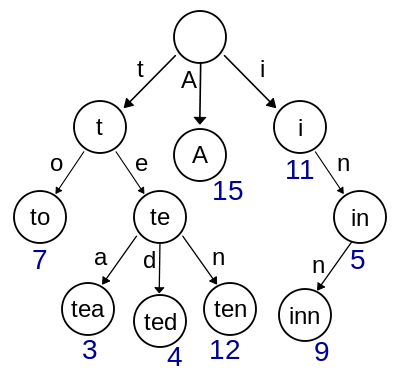
\includegraphics[width=0.3\textwidth]{trie1.png}
	\caption{Un trie de las claves "A", "to", "tea", "ted", "ten", "i",  "in", y "inn".}\label{figure}
\end{wrapfigure}
\large{
 Introducidos en 1959 independientemente por Rene de la Briandais1 y Edward Fredking, un trie es una estructura de datos de tipo árbol que permite la recuperación de información (de ahí su nombre del inglés reTRIEval). La información almacenada en un trie es un conjunto de claves, donde una clave es una secuencia de símbolos pertenecientes a un alfabeto. Las claves son almacenadas en las hojas del árbol y los nodos sirven para guiar la búsqueda.\\
 
 El árbol se estructura de forma que cada letra de la clave se sitúa en un nodo de forma que los hijos de un nodo representan las distintas posibilidades de símbolos diferentes que pueden continuar al símbolo representado por el nodo padre. Por tanto la búsqueda en un trie se hace de forma similar a como se hacen las búsquedas en un diccionario:\\
 
 Se empieza en la raíz del árbol. Si el símbolo que estamos buscando es A entonces la búsqueda continúa en el subárbol asociado al símbolo A que cuelga de la raíz. Se sigue de forma análoga hasta llegar al nodo hoja. Entonces se compara la cadena asociada a el nodo hoja y si coincide con la cadena de búsqueda entonces la búsqueda ha terminado en éxito, si no entonces el elemento no se encuentra en el árbol.
 
 Por eficiencia se suelen eliminar los nodos intermedios que sólo tienen un hijo, es decir, si un nodo intermedio tiene sólo un hijo con cierto carácter entonces el nodo hijo será el nodo hoja que contiene directamente la clave completa, se analiza este cambio en el apartado 1.2.}
\subsection{Definición formal}
\paragraph{}
\large{Un trie es un caso especial de autómata finito determinista (S,  $\Sigma$, T, s, A), que sirve para almacenar un conjunto de cadenas E en el que:

\begin{itemize}
	\item $\Sigma$ es el alfabeto sobre el que están definidas las cadenas.
	
	\item S, el conjunto de estados, cada uno de los cuales representa un prefijo de E.
	
	\item La función de transición: T : $S \times  \Sigma \to \mathcal S$; está definida como sigue: $ T(x,\sigma)=x\sigma$  si  $x, x\sigma \in S$, e indefinida en otro caso.
	
	\item El estado inicial s corresponde a la cadena vacía $\lambda$.
	
	\item El conjunto de estados de aceptación A $\subseteq$ S es igual a E.
	
\end{itemize}
	}
\subsection{Análisis y compresión de la estructura}
\large{
\paragraph{}
La situación general es la siguiente, el universo U esta compuesto de todos los strings de longitud \textit{l} sobre un alfabeto de digamos n elementos, U = $\{O,..., k-1\}^{l}$. Un conjunto S $\subseteq $ U está representado como un árbol k-ario compuesto por todos los prefijos de los elementos de S.\\

\begin{figure}[hbtp]
	\centering
	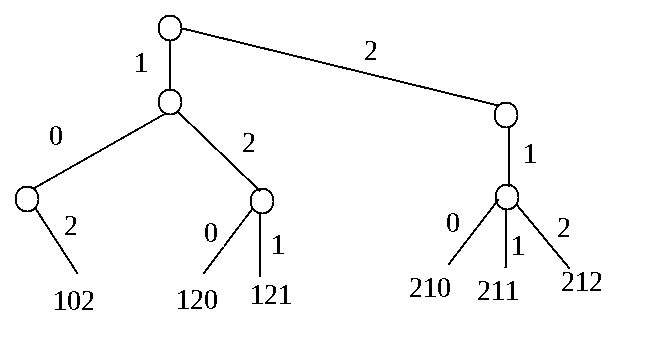
\includegraphics[width=0.4\textwidth]{trie2.png}
\end{figure}

La implementación más sencilla y que antes nos vendría a la mente sería utilizar un array de longitud n para cada nodo interno del árbol. La operaciones Acceder, Insertar y Eliminar serían muy rápidas y sencillas de programar. En particular si guardáramos el inverso de cada elemento de S ( en el ejemplo sería \{121, 201, 112, 021, 012, 212\}), entonces el siguiente programa serviría para realizar la operación:\\

Acceder(x)\\
	\hspace*{1.5cm} v $\leftarrow$  raiz;\\
	\hspace*{1.5cm} y $\leftarrow$ x;\\
	\hspace*{1.5cm} \textbf{hacer} \textit{l} \textbf{veces} ( i , y) $\leftarrow$ (y mod k, y div k);\\
	\hspace*{2.5cm}	v $\leftarrow$ i-ésimo hijo de v\\
	\hspace*{1.5cm} \textbf{fin};\\
	\hspace*{1.5cm} \textbf{si} x = CONTENIDO[v] \textbf{entonces} "Sí" \textbf{sino} "no"\\
	
Este programa toma tiempo O(\textit{l}) = O($\log_{k}N$) donde N = $|$U$|$. Desafortunadamente, el espacio requerido por un Trie como el descrito arriba puede ser enorme, del orden O(n$\cdot$\textit{l}$\cdot$k). Esto es, para cada elemento del conjunto S, $|$S$|$ = n, deberíamos guardar todo el recorrido de nodos, hasta \textit{l} nodos, y cada uno de estos tendría grado 1 y utilizaría espacio O(k). \\

Existe una forma más simple de reducir el espacio requerido a O(n$\cdot$k), eliminando el término \textit{l}. Consiste en eliminar los nodos de grado 1 y guardar nodos internos de grado 2 al menos. Puesto que un trie para un conjunto S de tamaño n tiene n hojas habrá como mucho n-1 nodos internos de grado 2 o más. Las cadenas de nodos de grado 1 se sustituyen por un único número, el número de nodos en la cadena. Si transformamos el ejemplo anterior obtenemos: \\

\begin{figure}[hbtp]
	\centering
	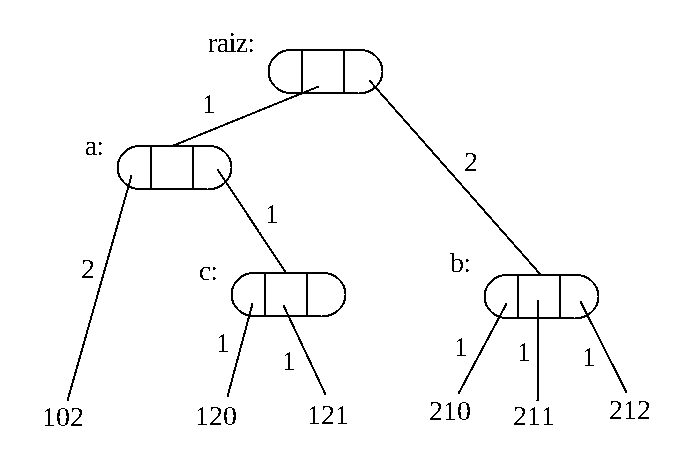
\includegraphics[width=0.6\textwidth]{trie3.png}
\end{figure}

Aquí los nodos internos están representados como arrays de longitud 3. En las flechas de padre a hijo está indicado el aumento en la profundidad del árbol, esto es 1 + el número de nodos eliminados. En el ejemplo el número 2 en la flecha que sale de la raíz, indica que en el hijo(b) hay que ramificar el tercer dígito (1 + 2). El algoritmo para Acceder, Insertar y Eliminar se complica ligeramente para Tries comprimidos pero sigue manteniendo el mismo orden.\\

Lo recién expuesto demuestra el siguiente teorema:\\

\textit{\textbf{Teorema:} Un Trie comprimido permite las operaciones Acceder, Insertar y Eliminar en tiempo O($\log_{k}N$), donde N es el tamaño del universo y k es el factor de ramificación del Trie. Un conjunto S de n elementos requiere espacio O(n$\cdot$k).}\\

Cabe destacar el interesante equilibrio espacio-tiempo que exhiben los Tries. Elegir un factor de ramificación k alto hará más rápido el Trie pero más costoso en términos de memoria, en cambio elegir un k pequeño hará más lenta la búsqueda pero requerirá menos memoria.
}
\pagebreak
\subsection{Tries estáticos}
\large{
\paragraph{}En esta sección se muestra a grandes rasgos como es posible reducir drásticamente el uso de memoria sin aumentar el tiempo de acceso. Los tries estáticos solo permiten la operación Acceder. La reducción se realiza en dos pasos. En el primer paso se utiliza una técnica general de solapamiento que sirve para comprimir tablas dispersas(sparse). Este primer paso reduce el espacio requerido a O(n log log n). En un segundo paso se reduce el espacio requerido hasta O(n) apilando varios números en un único espacio de memoria.\\

En nuestro ejemplo utilizaríamos un array de longitud 10 para almacenar los cuatro arrays de longitud 3 correspondientes a los nodos, y una tabla adicional para almacenar en que posición comienza de cada nodo.\\

\begin{figure}[hbtp]
	\centering
	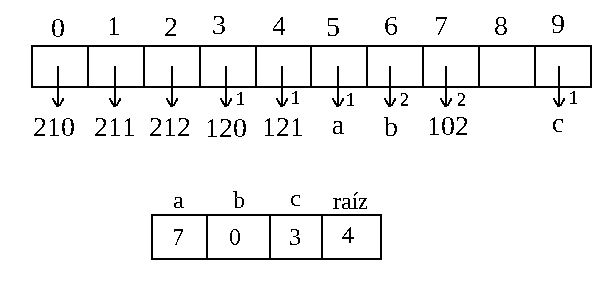
\includegraphics[width=0.7\textwidth]{trie4.png}
\end{figure}

Supongamos que buscamos el 121. Seguimos el primer apuntador (1) partiendo desde la raíz, el apuntador en la posición 4 + 1 en el array grande. Este nos lleva al nodo a. Seguimos el apuntador (2) desde a, es la posición 7 + 2 del array mayor que nos lleva al nodo c. Finalmente seguimos el apuntador 1 desde c que nos lleva a la posición 3 + 1, es una hoja, comparamos los valores y vemos que hemos hallado el 121.\\

Supongamos ahora que buscamos el 012, que no se halla en el Trie, seguimos el apuntador 0 desde la raíz, este nos lleva a la posición 4 + 0 que es una hoja, comparamos los contenidos y 121 $\neq$ 012 por lo que 012 no es miembro del conjunto.\\

Describiré ahora con algo más de detalle la técnica de compresión utilizada.
Sea A una matriz de r por s compuesta por ceros y unos con exactamente m entradas iguales a 1. Queremos hallar un pequeño desplazamiento de filas fd(i) tal que si guardamos la i-ésima fila de la matriz A en un array uni-dimensional en la posición fd(i) ningún par de unos colisione. En nuestro ejemplo los 0s corresponden a apuntadores nulos y los 1s a apuntadores no nulos. Un método para computar este desplazamiento de filas es el método decreciente del primero que mejor se ajusta( first-fit decreasing method).\\

\begin{enumerate}
	\item Ordena las filas de forma decreciente en función del número de unos. La fila con el número máximo de unos es la primera.
	
	\item Fija fd(0) = 0. Para i $\geq$ 1 elige rd(i) $\geq$ 0 mínimo tal que no ocurran colisiones con las filas colocadas previamente 0 a i - 1.
\end{enumerate}
}
\large{
En nuestro ejemplo el paso 1 podría producir la siguiente matriz.\\


\begin{figure}[hbtp]
	\centering
	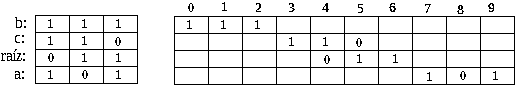
\includegraphics[width=1\textwidth]{trie5.png}
\end{figure}

En el paso 2 elegiríamos fd(0) = 0, fd(c) = 3, fd(raíz) = 4 y fd(a) = 7. Estas elecciones están ilustradas por la segunda matriz.\\

Para más detalle sobre Tries estáticos y una demostración completa de las técnicas expuestas y las demostraciones de los teoremas que las respaldan consultar \cite{key-2} apartado III. 1.2 STATIC TRIES or Compressing Sparse Tables.
}
\subsection{Ventajas}
\large{
	Las ventajas principales de los tries sobre los árboles de búsqueda binaria (BST) son:
\begin{itemize}
	\item búsqueda de claves más rápida. La búsqueda de una clave de longitud m tendrá en el peor de los casos un coste de O(m). Un BST tiene un coste de O(mlog n), siendo n el número de elementos del árbol, ya que la búsqueda depende de la profundidad del árbol, logarítmica con el número de claves.
	\item menos espacio requerido para almacenar gran cantidad de cadenas pequeñas, puesto que las claves no se almacenan explícitamente
	\item mejor funcionamiento para el algoritmo de búsqueda del prefijo más largo.
\end{itemize}}
\subsection{Aplicaciones}
\large{
Un Trie puede usarse para:

\begin{itemize}

	\item \textbf{Reemplazar una Tabla hash}, sobre la que presenta ventajas como que en un trie no se producen colisiones de claves, o no hay que definir una función de hash, o modificarla si añadimos más claves.
	\item \textbf{Como representación de diccionarios} Una aplicación frecuente de los tries es el almacenamiento de diccionarios, como los que se encuentran en los teléfonos móviles, cuando se necesita almacenar información adicional sobre las palabras, sino, un autómata finito determinista acíclico mínimo usa menos espacio que un trie.
	\item \textbf{Algoritmos de correspondencia aproximada}, como los usados en el software de corrección ortográfica.
\end{itemize}
}
\pagebreak
\section{Árbol de sufijos y array de sufijos}

\subsection{Árbol de sufijos}
\paragraph{}
Un árbol de sufijos representa la estructura interna de un string de una forma más profunda que otros algoritmos de preprocesamiento y de búsqueda de patrones. Un árbol de sufijos puede usarse para resolver el problema de búsqueda de la palabra exacta en tiempo linea, pero lo que lo hace interesante es su capacidad de resolver en tiempo lineal problemas de strings más complejos como la búsqueda inexacta o la búsqueda de la subcadena.\\

Dado un texto T de longitud m, tras O(m) tiempo de preprocesamiento, un árbol de sufijos es capaz de determinar en tiempo lineal O(n) si un string S de tamaño n está presente en T o no. Esto es, el coste de determinar si una palabra aparece en un texto depende de la longitud de la palabra y no del tamaño del texto, una vez realizado el preprocesamiento.

\subsubsection{Definición}
\paragraph{}
	Un árbol de sufijos \textit{T} para un string \textit{S} de \textit{m} caracteres es un árbol dirigido con exactamente \textit{m} hojas numeradas de 1 a \textit{m}. Cada nodo interno, distinto de la raíz, tiene al menos dos hijos y cada arista está etiquetada con una subcadena no vacía de \textit{S}. Dos aristas salientes de un mismo nodo no pueden tener subcadenas con el mismo caracter de comienzo. La funcionalidad clave del árbol de sufijos es que para cada hoja \textit{i}, la concatenación de las etiquetas de las aristas desde la raíz a la hoja es el sufijo de \textit{S} que comienza en la posición \textit{i}, esto es, \textit{S}[\textit{i..m}].\\
	
	La siguiente imagen muestra un árbol de sufijos para la cadena \textit{xabxac}:
	\begin{figure}[hbtp]
		\centering
		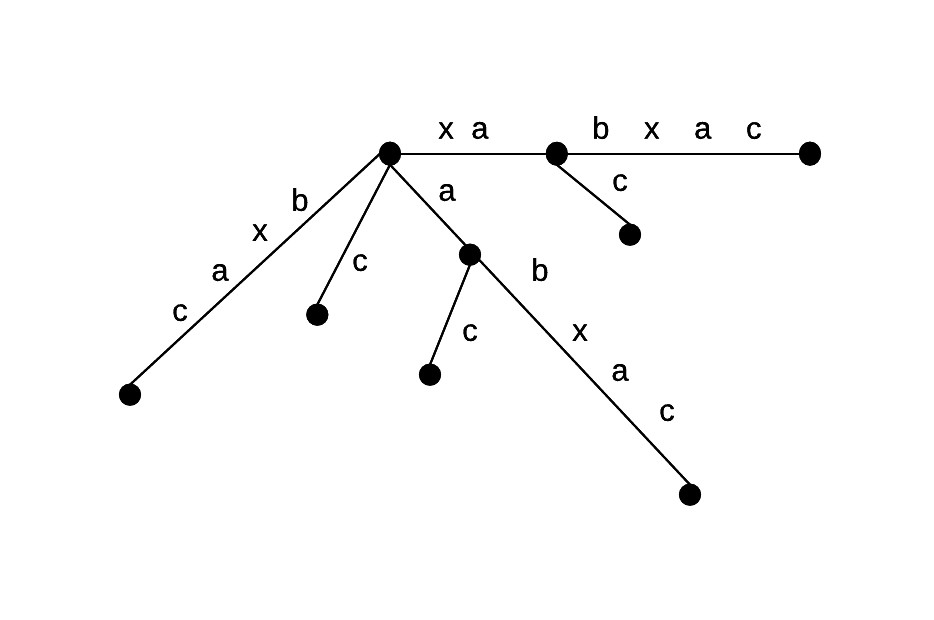
\includegraphics[width=0.6\textwidth]{SuffixTree1.png}
	\end{figure}
	
	Según la definición de arrriba no está garantizado que exista un árbol de sufijo para cualquier string S. El problema es que si un sufijo de S coincide con el prefijo de otro sufijo de S, entonces no es posible construir un árbol que respeta la definición expuesta ya que el camino del primer sufijo no terminaría en una hoja. Se puede evitar este problemas utilizando un caracter que no pertenezaca al alfabeto a modo de terminación.
	
\subsubsection{Aplicaciones}

\begin{itemize}
	\item Hallar la cadena exacta.
	\item Subcadena común más larga entre dos strings.
	\item Comprimir árboles de sufijos en DAGs, principalmente para reducir el uso del espacio.
	\item Hallar la coincidencia entre sufijo-prefijo más larga para cada par $S_{i},S_{j}$ en una colección de strings $S$.
	\item Reconocimiento de ADN contaminado.
	\item Reconocimiento de estructuras repetitivas en ADN y cadenas bilógicas.
\end{itemize}

\subsection{Array de sufijos}
\paragraph{}
Los arrays de sufijos fueron introducidos por Manber y Myers (1990) como una simple variante eficiente en espacio a los árboles de sufijos.\\

Un array de sufijos es un array ordenado de todos los sufijos de una cadena dada. Esta estructura de datos es muy simple, pero sin embargo es muy poderosa y es usada en algoritmos de compresión de datos y dentro del campo de la bioinformática , indización de textos completos, entre otros.

\subsubsection{Definición}
\paragraph{}
Sea $S=s_{1},s_{2},...s_{n}$ una cadena y sea $S[i,j]$ la subcadena de $S$ que va desde el índice $i$ hasta $j$.
El array de sufijos $A$ de la cadena $S$ va a ser un array de enteros brindando las posiciones iniciales de los sufijos de $S$ en orden léxico.Esto significa que $A[i]$ contiene la posición inicial del $i$-esimo sufijo más pequeño en $S$ y por tanto se cumple que para todo $1 < i\leq n: S[A[i-1],n] < S[A[i],n]$. Esto es, el sufijo en la posición \textit{Pos}(1) de S será el de menor valor léxico y en general el sufijo \textit{Pos}(\textit{i}) de S será léxicamente menor que el sufijo en \textit{Pos}(\textit{i} + 1) \\

Al igual que en el caso de los árboles es conveniente añadir un símbolo de fin de string como  puede ser $ $ \textdollar  $ $ al final de \textit{S}, y ahora interpretaremos que es de menor valor léxico que cualquier otro caracter en el alfabeto. \\

\pagebreak
El siguiente es un ejemplo de un array sufijo de la palabra \textit{mississippi}:\\

\hspace*{2cm}11:  i \\
\hspace*{2.6cm} 8:  ippi \\
\hspace*{2.6cm} 5:  issippi \\
\hspace*{2.6cm} 2:  ississippi \\
\hspace*{2.6cm} 1:  mississippi \\
\hspace*{2.6cm}10:  pi \\
\hspace*{2.6cm} 9:  ppi \\
\hspace*{2.6cm} 7:  sippi \\
\hspace*{2.6cm} 4:  sissippi \\
\hspace*{2.6cm} 6:  ssippi  \\
\hspace*{2.6cm} 3:  ssissippi \\

El array sufijo \textit{Pos} es 11, 8, 5, 2, 1, 10, 9, 7, 4, 6, 3.\\¸

Cabe destacar que el array solo contiene enteros y por lo tanto no almacena información sobre el alfabeto usado en la cadena S, por lo tanto el espacio requerido por una cadena de tamaño m es modesto y puede ser almacenado en exactamente m palabras de memoria, asumiendo que el tamaño de una palabra es al menos log m bits.

\subsubsection{Transformas árbol de sufijos en array de sufijos en tiempo lineal}

\paragraph{}
Suponiendo que disponemos del espacio suficiente para construir un árbol para S, un array de sufijos puede ser obtenido a partir de un árbol \textit{T} realizando una búsqueda "léxica" en profundidad de \textit{T}.\\

Definimos una arista (\textit{v}, \textit{u}) como léxicamente menor que otra arista (\textit{v}, \textit{w}) si y solo si el primer caracter de (\textit{v}, \textit{u}) es léxicamente menor que el primer caracter de (\textit{v}, \textit{w}). (El caracter de fin de string $ $ \textdollar  $ $ es léxicamente menor que cualquier otro).\\

Puesto que no hay dos aristas salientes del mismo nodo con el mismo caracter de comienzo, siempre existe un orden léxico estricto entre las aristas salientes de un nodo. Este orden implica que el camino desde la raíz de \textit{T} hasta la primera hoja que se alcance representará el sufijo de menor valor léxico. Por lo tanto el array de sufijos \textit{Pos} es una lista ordenada de los números de sufijos hallados en las hojas de \textit{T} durante la búsqueda en profundidad.\\

Dado que el árbol \textit{T} se construye en tiempo lineal y el recorrido se realiza también en tiempo lineal, podemos concluir que el array \textit{Pos} se construye en tiempo lineal O(\textit{m}) siendo \textit{m} el número de caracteres.\\

\pagebreak
\subsubsection{Reconocer patrones utilizando un array de sufijos}
\paragraph{}
El array de sufijos para una cadena \textit{S} permite con un simple algoritmo hallar todas las ocurrencias de cualquier patrón \textit{P} en \textit{S}. La clave del algoritmo se basa en una propiedad que dice que si \textit{P} está en \textit{S} entonces todas las posiciones en las que ocurre \textit{P} estarán agrupadas consecutivamente en \textit{Pos}.\\

Por ejemplo, \textit{P = issi} ocurre en \textit{mississippi} comenzando en la posición 2 y 5, que son adyacentes en \textit{Pos} (mirar ejemplo de anterior). Por lo tanto la búsqueda de ocurrencias de \textit{P} en \textit{S} se reduce a una búsqueda binaria a lo largo del array de sufijos. En mayor detalle, supongamos que \textit{P} es léxicamente menor que el sufijo en la posición del medio de \textit{S} (\textit{Pos}[\textit{m}/2]). En ese caso, de hallarse \textit{P} en \textit{S}, está necesariamente en la primera mitad de \textit{Pos}.\\

Utilizando la búsqueda binaria puede hallarse el menor índice \textit{i} en \textit{Pos}(si existe) tal que \textit{P} coincide exactamente con los \textit{n} primeros caracteres del sufijo \textit{Pos}(\textit{i}). De manera similar puede hallarse el mayor índice \textit{i}' con dicha propiedad, entonces el patrón \textit{P} sucederá en \textit{S} y comenzará en cada posicion dada por \textit{Pos}(\textit{i}) hasta \textit{Pos}(\textit{i}').\\

\textbf{Teorema} \textit{Utilizando la búsqueda binaria sobre el array \textit{Pos}, pueden hallarse todas las ocurrencias de \textit{P} en \textit{S} en tiempo O(n log m).}\\

\subsubsection{Mejora del algoritmo de reconocimiento de patrones}
\paragraph{}
Según se lleva a cabo la búsqueda binaria, denotemos por \textit{L} y \textit{R} los extremos del intervalo de búsqueda actual. Al inicio \textit{L} será 1 y \textit{R} será igual a \textit{m}. En cada iteración de la búsqueda se consulta la posición \textit{M} = $ \lceil(R + L)/2\rceil$ del array \textit{Pos}. El algoritmo de búsqueda guarda un registro de los prefijos más largos de \textit{Pos}(\textit{L}) y \textit{Pos}(\textit{R}) que coinciden con algún prefijo de \textit{P}, que denotaremos por \textit{l} y \textit{r} respectivamente, y sea \textit{mlr} = min (\textit{l}, \textit{r}).\\

Pueden utilizarse los valores \textit{mlr} para acelerar las comparaciones léxicas de \textit{P} y \textit{Pos}(\textit{M}). Ya que que los sufijos de \textit{S} están ordenados en el array \textit{Pos}, si \textit{i} es un índice entre \textit{L} y \textit{R}, los primeros \textit{mlr} caracteres del sufijo \textit{Pos}(\textit{i}) son necesariamente iguales que los primeros \textit{mlr} caracteres del sufijo \textit{Pos}(\textit{L}) y por lo tanto de \textit{P}. Esto quiere decir que a la hora de comparar \textit{P} con \textit{Pos}(\textit{M}) no es necesario empezar comparando desde la primera posición sino desde la posición \textit{mlr} + 1.\\

Mantener \textit{mlr} a lo largo de la búsqueda binaria añade ligeros costes adicionales al algoritmo pero evita realizar muchas comparaciones redundantes. Al comienzo de la búsqueda, cuando \textit{L} = 1 y \textit{R} = \textit{m}, es neceario compara \textit{P} con los sufijos \textit{Pos}(1) y \textit{Pos}(\textit{m}) para hallar \textit{l}, \textit{r} y \textit{mlr}. Sin embargo en el caso peor el algoritmo sigue siendo de orden O(n log m).\\

\subsubsection{Acelerando todavía más el algoritmo de reconocimiento de patrones}
\paragraph{}
Decimos que la examinación de un caracter es redundante cuando este ha sido examinado antes. El objetivo de la aceleración es reducir el número de comparaciones redundantes a como máximo una por cada iteración de la búsqueda binaria. El uso de \textit{mlr} por sí solo no es suficiente para alcanzar este objetivo. Puesto que \textit{mlr} es el mínimo entre \textit{l} y \textit{r}, cuando \textit{l} $\neq$ \textit{r}, todos los caracteres de P desde \textit{mlr} +1 hasta el máximo de \textit{l} y \textit{r} ya habrán sido examinados, y por lo tanto la comparación de dichos caracteres será redundante. Lo que es necesario es una manera de comenzar las comparaciones en el máximo de \textit{l} y \textit{r}.\\

Definamos \textit{Lcp}(\textit{i},\textit{j}) (Longes common prefix) como la longitud del prefijo más largo común a los sufijos en las posciones \textit{i} y \textit{j} de \textit{Pos}. \\

Por ejemplo, si \textit{S} = \textit{mississippi}, el sufijo \textit{Pos}(3) es \textit{issippi} y el sufijo \textit{Pos}(4) es \textit{ississippi}, por lo tanto \textit{Lcp}(3,4) = 4.\\

Para acelerar la búsqueda el algoritmo utiliza \textit{Lcp}(\textit{L},\textit{M}) y \textit{Lcp}(\textit{M},\textit{R}) para cada trio (\textit{L},\textit{M},\textit{R}) que surge durante la búsqueda binaria.\\

De esta manera es posible mejorar el órden del algoritmo a O(n + log m).\\

Para una demostración formal y más detalle sobre el uso de Lcp y como obtenerlo consultar \cite{key-3} apartados 7.14.4, 7.14.5.
\subsubsection{Aplicaciones}
\paragraph{}
Ha sido demostrado todo algoritmo de árbol de sufijos puede ser sistemáticamente reemplazado con un algoritmo que use un array de sufijos unido con información adicional (como un array de prefijos comunes) y resuelve el mismo problema y con la misma complejidad temporal.
\pagebreak

\begin{thebibliography}{arauak}
	
	\bibitem[NAVRAF]{key-5} GONZALO NAVARRO, MATHIEU RAFFINOT, Flexible pattern matching in strings
	
	\bibitem[MEHL]{key-2} KURT MEHLHORN, Data Structures and Algorithms 1: Sorting and Searching
	
	\bibitem[GUSFIELD]{key-3} DAN GUSFIELD, Algorithms on strings, trees, and secuences
	
	\bibitem[Wiki]{key-4} http://es.wikipedia.org/wiki/Arreglo\_de\_sufijos
	
	\bibitem[Wiki]{key-1} http://es.wikipedia.org/wiki/Trie
	
\end{thebibliography}

\end{document}
